\NextFile{StrategyModules.html}
\chapter{Strategy Modules}


These are modules that can be used via the syntax
\begin{lstlisting}{language=XML}
<module name="strategy" >
	<param name="ModuleProbability_1" value="0.1" />
	<param name="Module_1" value="ChangeLegMode" />
        <param name="ModuleProbability_2" value="0.1" />
        <param name="Module_2" value="TimeAllocationMutator" />
</module>
\end{lstlisting}


Strategy modules are numbered. Also, each  module is given a weight which determines the probability by which the  course of action represented by the module is taken. In this example,  each person stands a chance of 1/2 that their transport mode is changed,  and a chance of 1/2 that their time allocation is changed. (The  weights are renormalized so that they add up to one.)

A strategy module is, in the code, always a combination of a plan  selector and zero or more strategy module elements. There are two cases,  which are handled differently:
\begin{itemize}
	\item If there are zero strategy module elements, the chosen plan is made "selected" for the person, and the method returns.
	\item If there is at least one strategy module element, the chosen plan is  copied, that copy is added to the persons's set of plan, and the new  plan is made "selected". That new plan is then given to the  strategy module elements for modification. These latter strategy  modules, with at least one strategy module element, are sometimes called  "innovative".
\end{itemize}

The strategy modules that are understood by MATSim are defined in the class \href{http://www.matsim.org/xref/org/matsim/core/replanning/StrategyManagerConfigLoader.html}{StrategyManagerConfigLoader}. In addition, you can program your own strategy modules; see tutorial.programming in matsim/src/main/java for examples.

Unfortunately, the naming in the code is different from the naming in the config file:
\begin{itemize}
	\item "strategy" in config file --$>$ StrategyManager (or "set of strategies") in code
	\item "strategy module" in config file --$>$ PlanStrategy in code
	\item There is a PlanStrategyModule in the code; it corresponds to what was called strategy module element in the description above.
\end{itemize}

It is not clear which combinations of these modules can be used  together. Depending on required features, special variants sometimes  need to be used. This has not yet been sorted out. Also see \href{http://matsim.org/node/690}{here}.


\vfill\eject
\section{Selectors}

\subsection{BestScore.  Status: works}

Pure plan selecting (i.e. non-innovative) strategy module.

Will select the plan with the highest score. The score will be updated after execution of the mobsim.

Disadvantage: Will never try again plans that obtained a bad score  from a fluctuation (e.g. a rare traffic jam). It is therefore  recommended to either use this in conjunction with a small probability  for RandomPlanSelector, or to use ChangeExpBeta.

\subsection{ChangeExpBeta. Status: works. RECOMMENDED!}

\subsection{KeepLastSelected. Status: works}

\subsection{SelectExpBeta. Status: works}

Multinomial logit model choice between plans.

The scores are taken as utilities; the betaBrain parameter from the  config file is taken as the scale parameter. As equation:
\begin{verbatim}
p_i = exp( beta_brain * score_i) / sum_j exp( beta_brain * score_j )
\end{verbatim}

\subsection{SelectRandom}

\vfill\eject
\section{Innovative modules}


Divider: Pure plan selectors above, innovative strategy modules below.

\subsection{ReRoute.  Status: nearly indispensable}

\textbf{Maintainer:} Marcel Rieser

All routes of a plan are recomputed.

The module is called by inserting the following lines into the "strategy" module:
\begin{verbatim}
$<$module name="strategy" $>$
	$<$param name="ModuleProbability_XXX" value="0.1" /$>$
	$<$param name="Module_XXX" value="ReRoute" /$>$
                ...
$<$/module$>$
\end{verbatim}

The corresponding configuration module unfortunately has a different name:
\begin{verbatim}
$<$module name="planscalcroute" $>$
	$<$param name="beelineDistanceFactor" value="1.3" /$>$
	$<$param name="bikeSpeed" value="4.166666666666667" /$>$
	$<$param name="ptSpeedFactor" value="2.0" /$>$
	$<$param name="undefinedModeSpeed" value="13.88888888888889" /$>$
	$<$param name="walkSpeed" value="0.8333333333333333" /$>$
$<$/module$>$
\end{verbatim}

This works pretty reliably for car.

It also works for other modes, as "pseudo"-mode, in the following way:
\begin{itemize}
	\item Travel times for these other modes are not obtained from true  routing on the corresponding network, but by some estimates. These  are configured by the parameters above, but no guarantee that they work  consistently.
	\item The mobsim will not execute such routes on the network, but "teleport" them.
	\item The scoring works quite normally, since it just takes the time from leg start to leg end by mode.
\end{itemize}

It is possible to route such legs on the network, by using a different router.

It is \emph{not} possible to "physically" execute a leg in the  mobsim if it has not been routed before. That is, the capability  of the router needs to be $>$= the capability of the mobsim.  (Makes sense, if one thinks about it.)

\subsection{TimeAllocationMutator.  Status: works for vsp and ivt}

Simple  module that shifts activity end times randomly. ("Good" time  shifts will be selected through the matsim plans selection mechanism.)

The maximum extent of the shifts can be configured; see the config  section of the log file. It is, as of now (may'10), not possible  to add a comment to that parameter.

The usage of the module is configured in the "strategy" section.

\subsection{ ChangeSingleLegMode. Status: works}

\textbf{Maintainer:} Marcel Rieser

This replanning module randomly picks one of the plans of a person and changes the mode of transport of \textbf{one single leg}. The leg is picked randomly. For changing the mode of transport for all legs use \href{http://www.matsim.org/node/387}{ChangeLegMode}. In contrast to \href{http://www.matsim.org/node/387}{ChangeLegMode},  ChangeSingleLegMode allows for multiple modes in one plan. By default,  the supported modes are driving a car and using public transport. Also,  this module is able to (optionally) respect car-availability.

Note that the configuration is done by $<$module  name="changeLegMode"$>$ and not by $<$module  name="changeSingleLegMode"$>$. The replanning module is configured like  this using the very same configuration module as \href{http://www.matsim.org/node/387}{ChangeLegMode}:
\begin{verbatim}
$<$module name="changeLegMode"$>$
   $<$param name="modes" value="car,pt,bike,walk" /$>$
   $<$param name="ignoreCarAvailability" value="false" /$>$
$<$/module$>$
\end{verbatim}

Add the module to the replanning strategy like this:
\begin{verbatim}
$<$param name="Module_X" value="ChangeSingleLegMode" /$>$
$<$param name="ModuleProbability_X" value="0.1" /$>$
\end{verbatim}

Replace the 'X' with the number you assign to this module. For some more details on the syntax of this section, see \href{http://matsim.org/node/478}{here}.


By default, the simulation will handle legs with modes different from  "car" by using a delayed teleportation. If another behavior is  requested (e.g. detailed simulation of public transport), this needs to  be manually configured for the simulation.


\subsection{ChangeLegMode. Status: works}


\textbf{Maintainer:} Michael Zilske

This replanning module randomly picks one of the plans of a person  and changes its mode of transport.By default, the supported modes  are driving a car and using public transport. Only one mode of transport  per plan is supported. For using different modes for sub-tours on a  single day see the "SubtourModeChoice" module. Also, this module is able  to (optionally) respect car-availability.

The replanning module is configured like this, where the value  parameter lists the modes of transport from which the module randomly  chooses:
\begin{verbatim}
$<$module name="changeLegMode"$>$
   $<$param name="modes" value="car,pt,bike,walk" /$>$
   $<$param name="ignoreCarAvailability" value="false" /$>$
$<$/module$>$
\end{verbatim}

Add the module to the replanning strategy like this:
\begin{verbatim}
$<$param name="Module_X" value="ChangeLegMode" /$>$
$<$param name="ModuleProbability_X" value="0.1" /$>$
\end{verbatim}

Replace the 'X' with the number you assign to this module. For some more details on the syntax of this section, see \href{http://matsim.org/node/478}{here}.

By default, the simulation will handle legs with modes different from  "car" by using a delayed teleportation. If another behavior is  requested (e.g. detailed simulation of public transport), this needs to  be manually configured for the simulation.

This module can be used with the detailed simulation of public transport by changing the line

$<$param name="Module\_X" value="ChangeLegMode" /$>$

to

$<$param name="Module\_X" value="TransitChangeLegMode" /$>$

\subsubsection{Reference}

M. Rieser, D. Grether, K. Nagel;\textbf{Adding mode choice to a multi-agent transport simulation}; TRB'09

\subsection{LocationChoice. Status: ready}

\subsubsection{{Maintenance and Questions}}

A. Horni, IVT (horni\_at\_IVT.baug.ethz.ch)

\subsubsection{{Javadoc}}

\href{http://www.matsim.org/javadoc/org/matsim/locationchoice/package-summary.html}{www.matsim.org/javadoc/org/matsim/locationchoice/package-summary.html}



%%\subsubsection{{\textbf{Config Parameters\hypertarget{parameters}{}}}}
\subsubsection{Config Parameters}


\href{http://www.matsim.org/javadoc/org/matsim/locationchoice/package-summary.html#locationchoice_parameters}{www.matsim.org/javadoc/org/matsim/locationchoice/package-summary.html\#locationchoice\_parameters}



\subsubsection{{Status}}

Ready

\subsubsection{{In Brief}}

MATSim provides destination choice based on three  different basic concepts. First, random search can be applied. Second,  local search implemented in the time geography framework is available  [1]. Third, the most recent module ist best response and includes random  error terms to make MATSim fully compatible with discrete choice theory  [2]. The authors recommend to use this recent module in general. Random  search should be utilized for algorithmic comparative investigations  only.

The time geography module provides the possibility to  take into account spatial competition in the activity location  infrastructure (see Fig.~\ref{fig:locachoice:3}). It is planned-after a thorough calibration-to integrate spatial competition in the best response version.

Estimation of a MATSim destination choice utility function for Switzerland is in development [3].
% EndFragment




\subsubsection{{Calling the Location Choice Strategy}}

The strategy module in the config file needs to be extended as follows:
\begin{verbatim}
$<$module name="strategy"$>$
    ...
    $<$param name="ModuleProbability_X" value="0.0 $<$ double $<$=1.0" /$>$
    $<$param name="Module_X" value="LocationChoice" /$>$
    ...
$<$/module$>$
\end{verbatim}


\subsubsection{{I. Random Search}}

Due to slow convergence, this approach is only useful for very small scenarios.


\subsubsection{{II. Local Search With Time Geography}}

The MATSim local search destination choice module is  based on Hägerstrand's time geography. That is, in every replanning step  locations are chosen within the region restrained by travel time  budgets as defined by the time allocation module (see Fig.~\ref{fig:locachoice:1} and Fig.~\ref{fig:locachoice:2}). Within this region the choice is performed based on the MATSim utility function.

In more detail, the following procedure is  iteratively applied. An approximate choice set of locations is built to  begin with, where the constructing of this set is initially based on an  initial global travel speed assumption (\emph{recursionTravelSpeed}).  After tentatively choosing one location from this approximate set, the  actual accessibility in terms of travel time is checked. If the location  is not accessible it is rejected, the initial travel time is adapted  according to the \emph{recursionTravelSpeedChange}parameter  in the configuration file and a next trial is started. After a certain  number of failed trials to find an accessible location (\emph{maxRecursions}), the choice is made from the universal choice set.

The parameters \emph{recursionTravelSpeed}, \emph{recursionTravelSpeedChange}and \emph{maxRecursions }are explained in Section \hyperlink{parameters}{Parameters}


\subsubsection{{III. Best Response Including Random Error Terms}}

The parameters \emph{scaleEpsShopping }and \emph{scaleEpsLeisure }correspond to f$_Shopping$ and f$_Leisure$ in [2]. \emph{probChoiceSetSize }is $\Phi$, epsilonDistribution, \emph{tt\_}\emph{approximationLevel}, \emph{maxDistanceEpsilon}, and \emph{probChoiceExponent }are explained in in Section \hyperlink{parameters}{Parameters}.

The parameters \emph{scaleEpsShopping }and \emph{scaleEpsLeisure }can be calibrated, based on e.g., travel distance distributions as described in [2].

NOTE: This  variant will NOT work as described in Ref. [2] when configuring it as  described above. Additionally, the scoring function needs to be  modified. As of now, there does not seem to be a way to achieve  this without some Java programming. kai, jan'13

\subsubsection{{Spatial Competition: Facility Load Penalty Computation}}

Similar to route and time choice being influenced by  the competition in transport infrastructure it can be expected that  competition in activities infrastructure has an effect on destination  choice. Consequently, the utility of performing an activity is dependend  on the actual load of the activities infrastructure at least for some  activities such as e.g., grocery shopping (e.g.; searching for a parking  space or waiting time at cash points etc.). In MATSim spatial  competition is taken into account, which has shown to reduce the number  of implausibly overcrowded locations (see \hyperlink{Figure3}{Figure 3} below).

The score for perfoming an activity is calculated as follows:
\[
score = (1- fp) * score\_without\_penalty
\]
\[
fp = Max(0.5, fcrf)
\]
\[
fcrf = restraintFcnFactor * [(facility load) / (facility capacity)]^{restraintFcnExp}
\]
The parameters \emph{restraintFcnFactor}and \emph{restraintFcnExp }are explained in the section \hyperlink{parameters}{Parameters}


\subsubsection{{Literature}}

[1] Horni, A., D.M. Scott, M. Balmer and K.W. Axhausen (2009)  Location choice modeling for shopping and leisure activities with  MATSim: Combining micro-simulation and time geography, \emph{Transportation Research Record}, \textbf{2135}, 87-95.

[2] Horni, A., K. Nagel and K.W. Axhausen (2011) High-Resolution Destination Choice in Agent-Based Demand Models, \emph{Arbeitsberichte Verkehrs- und Raumplanung}, \textbf{682}, IVT, ETH Zürich, Zürich.

[3] Horni, A., D. Charypar and K.W. Axhausen (2011) Empirically  approaching destination choice set formation, paper presented at the \emph{90$^th$ Annual Meeting of the Transportation Research Board}, Washington, D.C., January 2011.

\subsubsection{Figures}

\begin{figure}
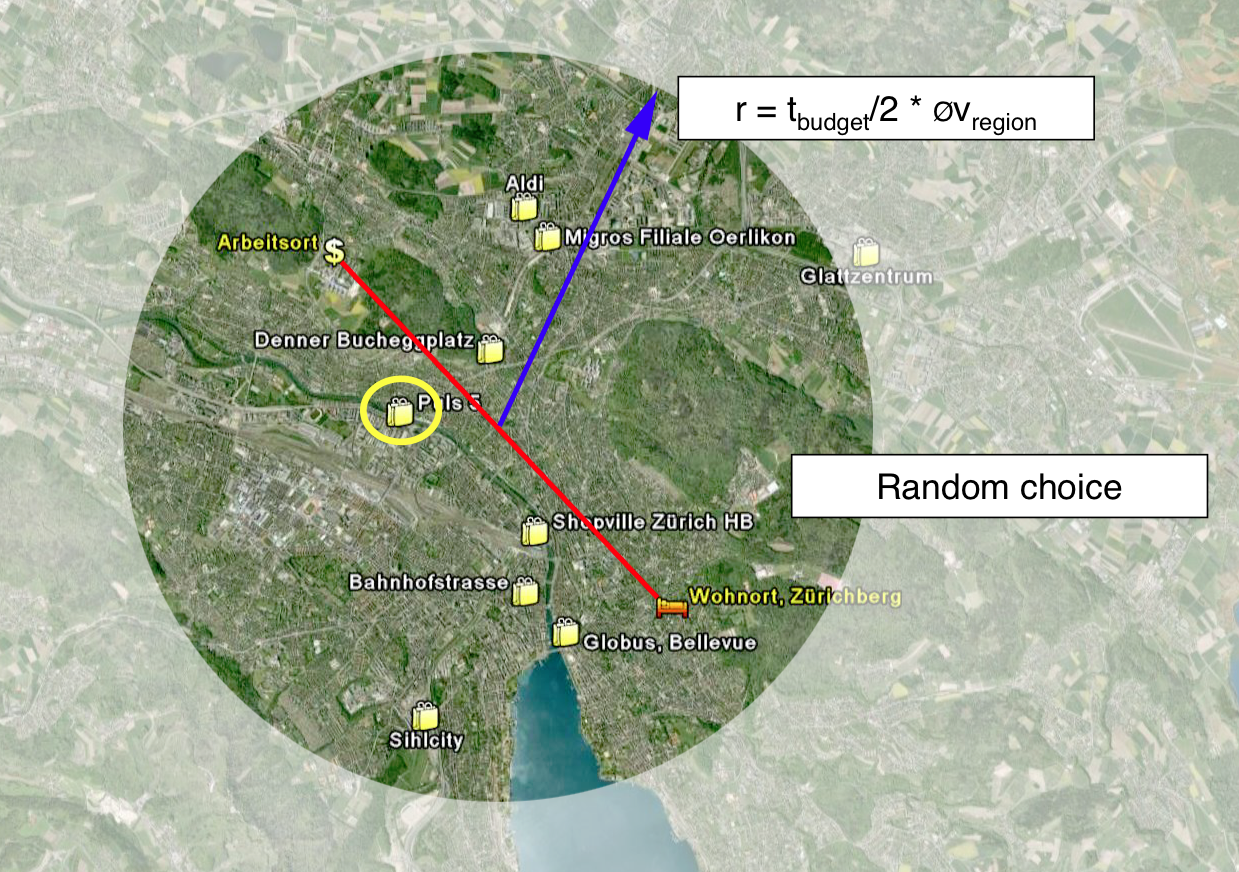
\includegraphics[width=.9\textwidth]{figures/locationChoice/locachoice1.png}
\caption{Region restrained by travel time budget}
\label{fig:locachoice:1}
\end{figure}

\begin{figure}
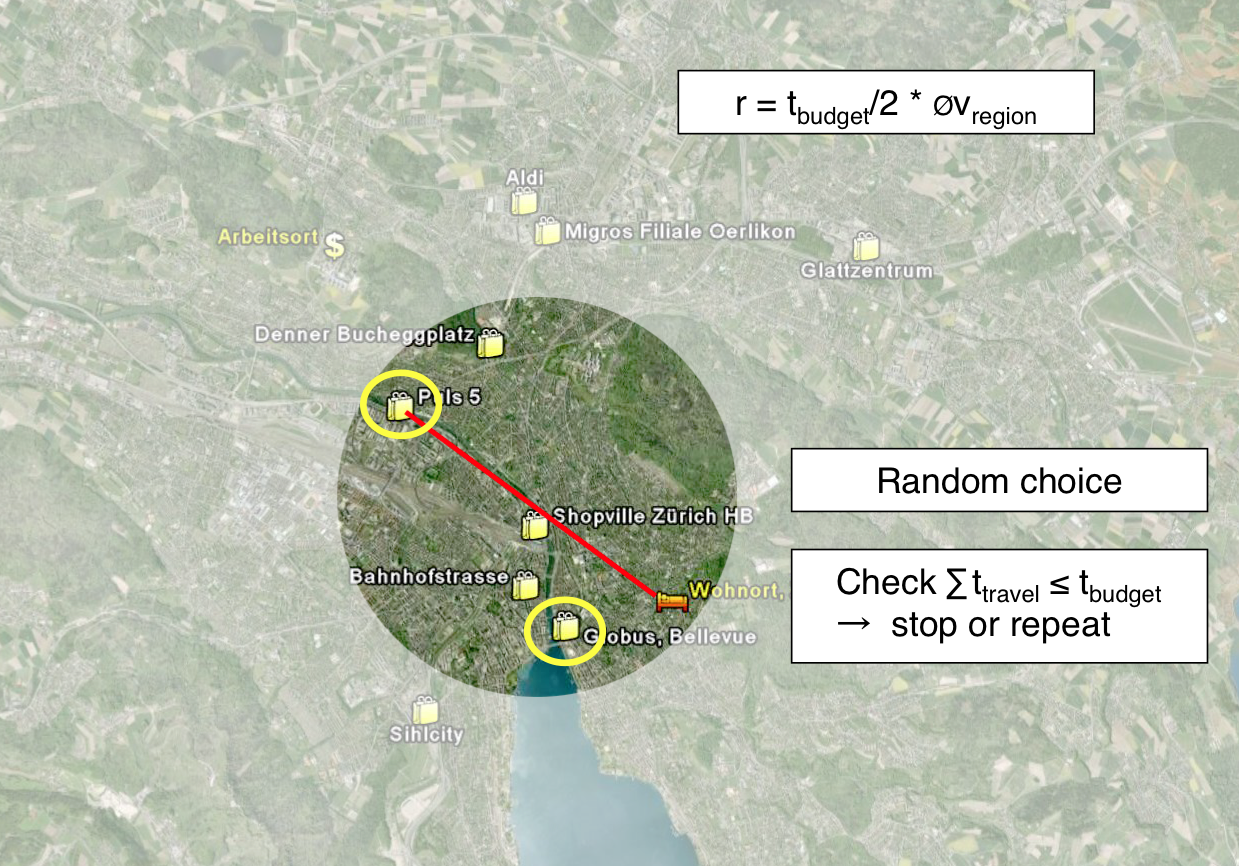
\includegraphics[width=.9\textwidth]{figures/locationChoice/locachoice2.png}
\caption{Region restrained by travel time budget}
\label{fig:locachoice:2}
\end{figure}

\begin{figure}
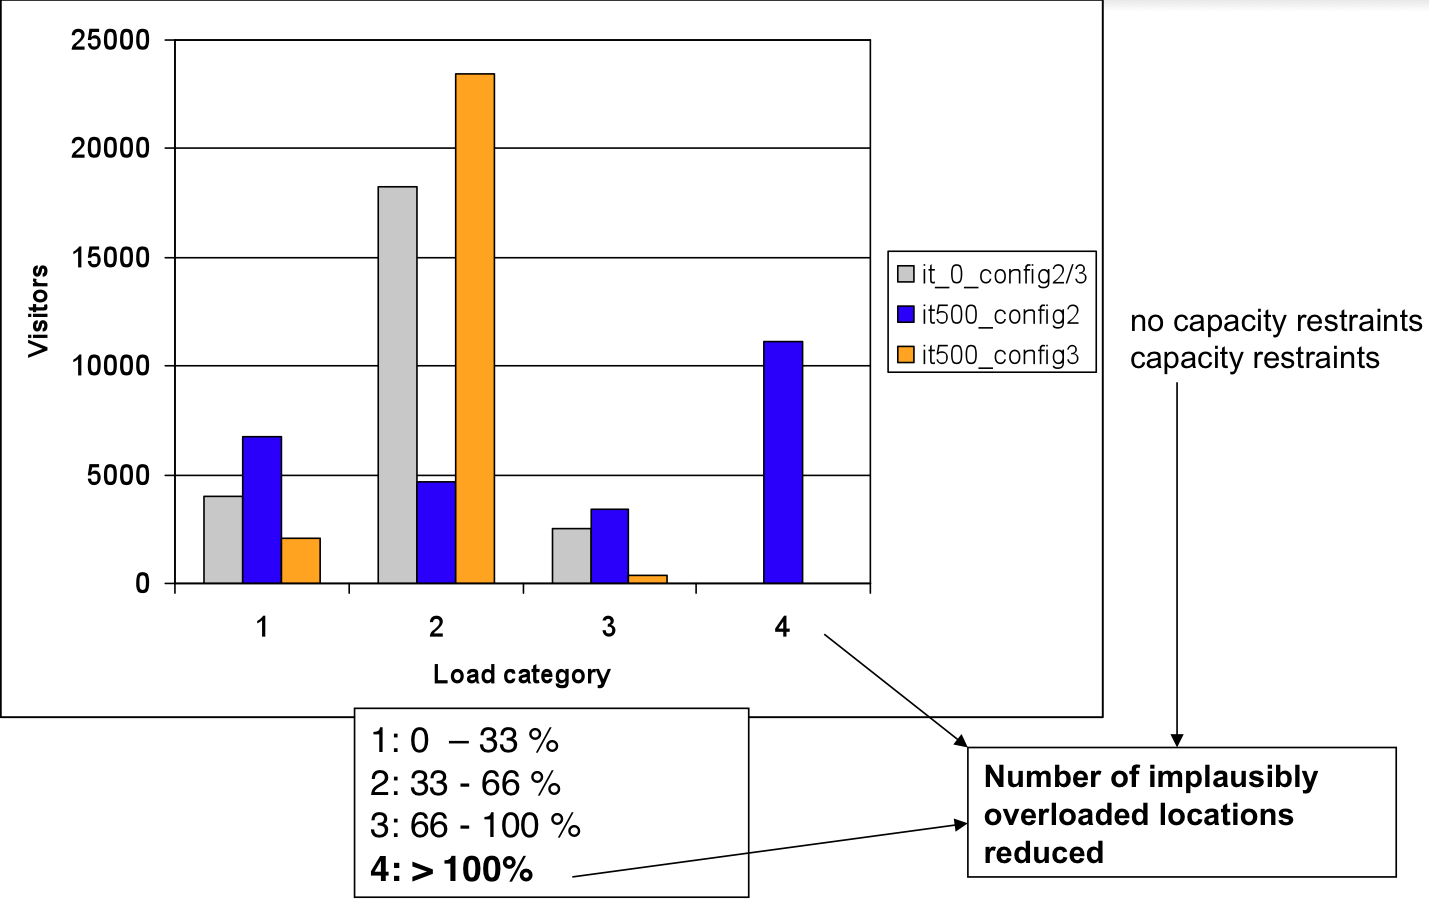
\includegraphics[width=.5\textwidth]{figures/locationChoice/locachoice_capacities.png}
\caption{Taking spatial competition into account}
\label{fig:locachoice:3}
\end{figure}






\subsection{SubtourModeChoice. Status: probably works}

\textbf{Maintainer:} Michael Zilske

In contrast to "ChangeLegMode", which changes \emph{all} legs of a plan to a different mode, this module changes the modes of sub-tours separately.

For example, somebody might take the car to work, walk to lunch and back, and take the car back home.

"chainBasedModes" means modes where a vehicle (car, bicycle,  ...) is parked and in consequence needs to be picked up again.
\begin{verbatim}
	$<$module name="subtourModeChoice" $>$
		$<$param name="chainBasedModes" value="car, bike" /$>$
		$<$param name="modes" value="car, bike, pt, walk" /$>$
	$<$/module$>$

\end{verbatim}

The module is called by inserting the following lines into the "strategy" module:
\begin{verbatim}
	$<$module name="strategy" $>$
		$<$param name="ModuleProbability_XXX" value="0.1" /$>$
		$<$param name="Module_XXX" value="SubtourModeChoice" /$>$
                ...
        $<$/module$>$

\end{verbatim}


For modes other than car, travel time and travel distance are  computed according to some heuristics, which are configured in the  router.

\vfill\eject
\section{Combination of strategy modules}

It  is not clear which combinations of these modules can be used together.  Depending on required features, special variants sometimes need to be  used. This has not yet been sorted out.

The following table tries to give an overview, but it is an old table  that has not been maintained (table status 2011; this sentence written  2012).
\begin{center}
\begin{tabularx}{\hsize}{|X|l|l|X|}
\hline 
\textbf{Choice dimension} & \textbf{Default Strategy} & \textbf{Transit} & \textbf{Transit \& Parking} \\ 
\hline
departure time choice & TimeAllocationMutator & TransitTimeAllocationMutator & ? \\ 
\hline
route choice & ReRoute & ReRoute & ? \\ 
\hline
mode choice
\\     (all legs get same mode) & ChangeLegMode & TransitChangeLegMode & ? \\ 
\hline
mode choice
\\     (each leg can have a different mode) & ChangeSingleLegMode & TransitChangeSingleLegMode & ? \\ 
\hline
mode choice
\\     (subtour-based) & SubtourModeChoice & TransitSubtourModeChoice & ? \\ 
\hline
location choice & LocationChoice & ? & ? \\ 
\hline
 &  &  &  \\ 
\hline
 &  &  &  \\ 
\hline
 &  &  &  \\ 
\hline

\end{tabularx}
\end{center}

Legend:
\begin{itemize}
	\item n/a means this choice dimension is not supported/available for the specified feature
	\item ? means there is no known implementation available
\end{itemize}
